\documentclass[11pt]{report}
\usepackage[margin=1in]{geometry}
\usepackage{titlesec}
\usepackage{graphicx}
\usepackage{parskip}
\usepackage{glossaries}
\usepackage{datetime}

\titleformat{\chapter}{\Large\bfseries}{}{0pt}{\huge}
\titlespacing\chapter{0pt}{*1}{*1}
\titlespacing\section{0pt}{*0}{-\parskip}
\titlespacing\subsection{0pt}{*0}{-\parskip}
\titlespacing\paragraph{0pt}{*0}{*3}

\newcommand*{\TitleFont}{
      \usefont{\encodingdefault}{\rmdefault}{b}{n}
      \fontsize{24}{36}
      \selectfont
}
\newcommand{\thickline}{\rule{\textwidth}{1.6pt}}
\newcommand{\thinline}{\rule{\textwidth}{0.4pt}}
\newcommand{\novspace}{\vspace*{-\baselineskip}\vspace*{4pt}}
\renewcommand{\dateseparator}{-}
\let\oldtitle\title
\renewcommand{\title}[1]{\oldtitle{\thickline \\ \novspace \thinline \\ \TitleFont {#1} \thinline \\ \novspace \thickline}}
\newcommand{\tableoffiguresandtables}{\listoffigures\begingroup\let\clearpage\relax\listoftables\endgroup}

\author{
	Evan Milton \\
	Computer and Electronics Engineering \\
	University of Nebraska at Lincoln - Omaha Campus \\
	Electronics Engineering
		\and
	Josh DeWitt \\
	Computer and Electronics Engineering \\
	University of Nebraska at Lincoln - Omaha Campus \\
	Computer Engineering and Mathematics, minor in Computer Science
		\and
	Chad Staley \\
	Computer and Electronics Engineering \\
	University of Nebraska at Lincoln - Omaha Campus \\
	Electronics Engineering
		\and
	James Gehringer \\
	Computer and Electronics Engineering \\
	University of Nebraska at Lincoln - Omaha Campus \\
	Computer Engineering, minor in Computer Science
}
\date{\yyyymmdddate\today}

\newacronym{2d}{2-D}{Two-Dimensional}
\newacronym{3d}{3-D}{Three-Dimensional}
\newacronym{arm}{ARM}{Advanced RISC Machines}
\newacronym{cnc}{CNC}{Computer Numerical Control}
\newacronym{dvi}{DVI}{Digital Visual Interface}
\newacronym{gpio}{GPIO}{General Purpose Input/Output}
\newacronym{led}{LED}{Light Emitting Diode}
\newacronym{lrc}{LRC}{Linear Responsibility Chart}
\newacronym{pcb}{PCB}{Printed Circuit Board}
\newacronym{pi}{Pi}{Raspberry Pi}
\newacronym{wbs}{WBS}{Work Breakdown Structure}
\newacronym{xp}{XP}{Extreme Programming}

\title{CNC Interface \\ Project Plan}

\begin{document}
\maketitle
\tableofcontents
\tableoffiguresandtables

\chapter{Project Definition}
The purpose of this Senior Thesis Project is to create a \gls{cnc} interface, capable of receiving standardized G-code through \gls{tcpip}, processing the G-code, and driving motors and \gls{gpio} according to the G-code. 

\section{Project Need}
The modern \gls{cnc} interface is limited to utilization of a full computer system, in combination with a motor driver platform to for complete functional control.
This setup can cost upwards of \$500, depending on the quality and system specifications.
This system will encapsulate these hardware and software requirements completely for less than \$100, bringing the \gls{cnc} interface to a price point comparable with that of the modern printer. 

\section{Existing Solutions}
\gls{cnc} system requirements currently rely upon complex computer-driver interfaces to control the machine.
The system requires a complete software package operating from a PC to manipulate an entirely separate set of motor drives running the machine.
While this may be practical for commercial and industrial applications, many of the features provided by this system will not be utilized by the average consumer.

\section{Existing Solutions Improvement}
This project will encapsulate these hardware and software requirements completely within a system costing less than \$100.
In combination of the basic functions provided by the PC with the root functionality of the motor driver unit, the system as a whole can be greatly simplified.
The addition of a Web-Interface will allow for users to operate the \gls{cnc} remotely.
This will bring system functionality to a level on par with the modern printer.

\section{Project Scope}
The \gls{cnc} interface will be configurable to operate on different mechanical systems. 
The scope includes the software for the G-code interpretation, its upload interface, the master controller, the motor controller and the motor driver board.
The G-code interpretation software will have a G-code file as an input and output motor driver commands from the master controller to the motor controller.
The motor controller will send out the driver signals to the motor driver board. 
The motor driver board will take the command outputs from the motor controller and then drive the motors. 
There will be 16 \gls{gpio} pins, an emergency stop switch, and home switches for the motors. 

\section{Marketing Requirements}
The system will meet the following criteria:
\begin{enumerate} \parskip2pt
	\item be accurate in its motor control.
	\item be able to quickly accelerate the motors.
	\item be able to send command files through a web interface.
	\item be able to drive multiple motors.
	\item be able to handle general purpose input and output.
	\item be able to be stopped in an emergency.
	\item be able to shutdown if the system gets too hot. 
	\item be able to operate at a range of input voltages.
\end{enumerate}

\section{Objective Tree}
~\ref{fig:o-tree} outlines the requirements for having a functioning \gls{cnc} interface for this Senior Thesis Project.
Safety is the most important objective in this project since the \gls{cnc} interface will control moving components, although these moving components are outside the scope of this report.
Next most important is the \gls{cnc} functionality, otherwise the interface would not be able to control any \gls{cnc}
Speed and accuracy is rated next most important to ensure the movements coordinated by the interface are as closed to the desired as possible.
The \gls{cnc} control is required to allow G-Code to be uploaded to the system and allow system monitoring.
A variable power input is desired so that users may purchase a power supply that fits their motors' needs, ensuring that a properly priced power supply is bought for the system.

\begin{figure}[H]
\centering
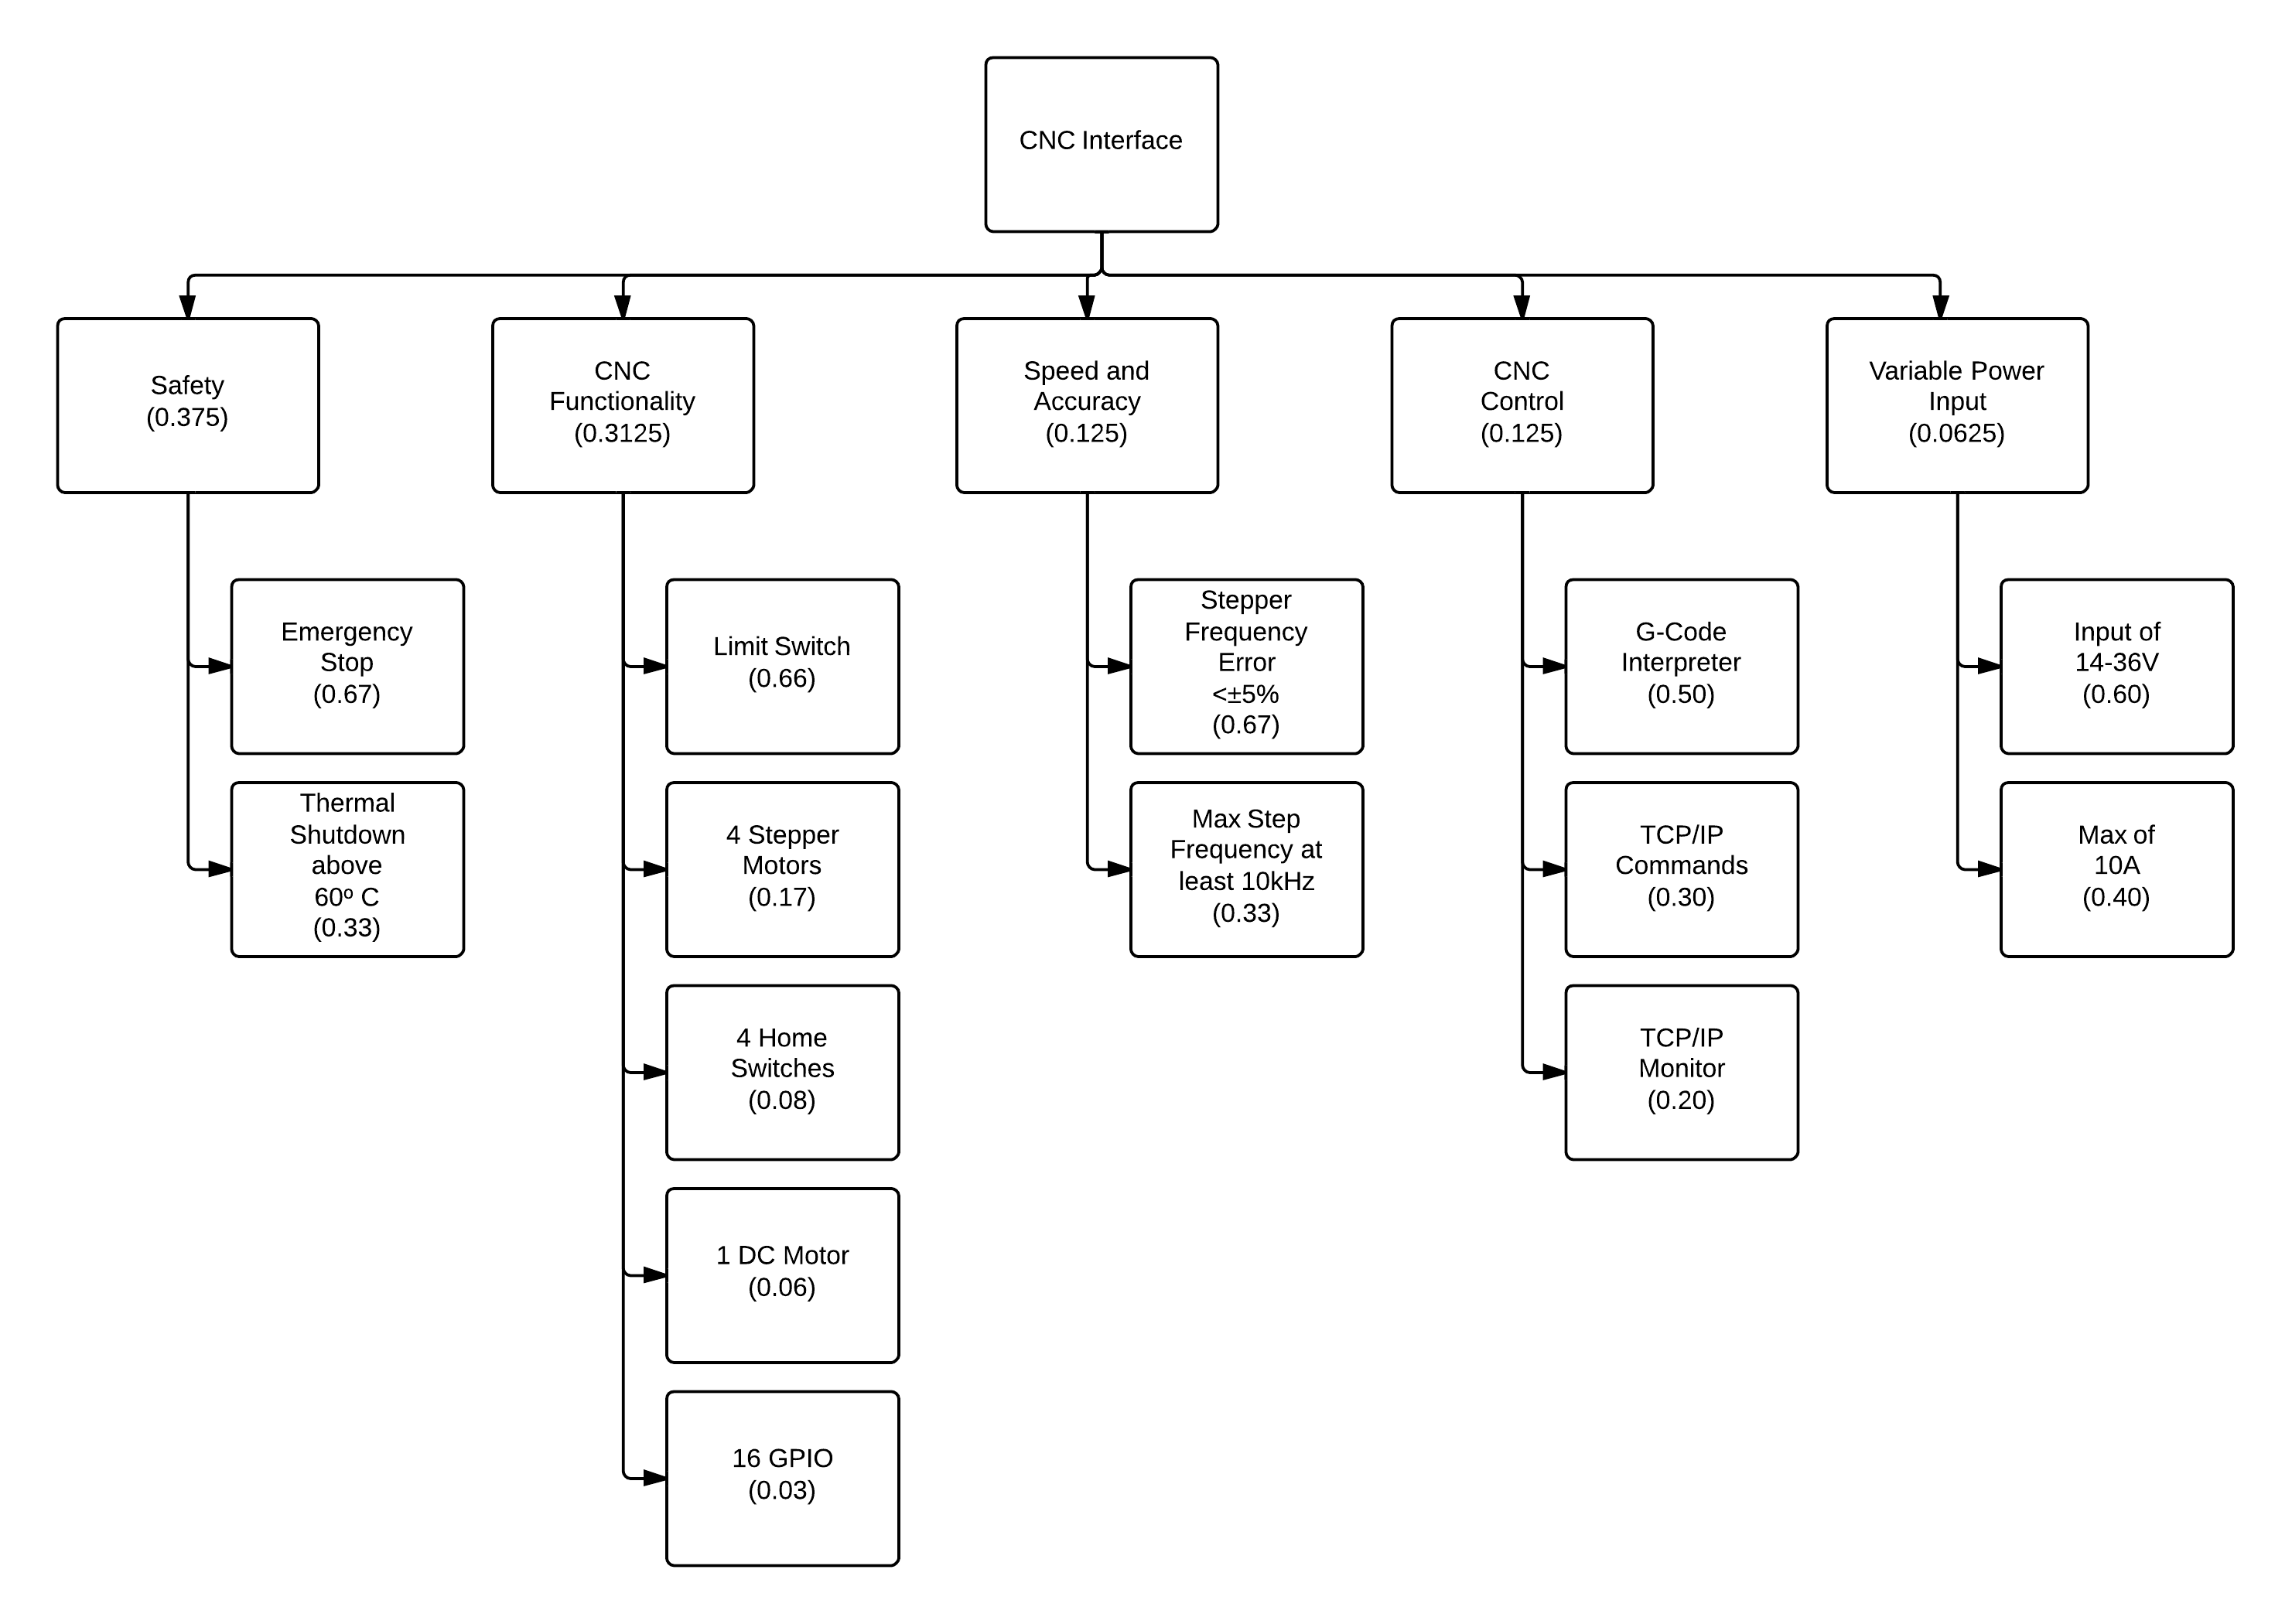
\includegraphics[width=1.0\textwidth]{otree.png}
\caption{Objective Tree}
\label{fig:o-tree}
\end{figure} 

\section{CEEN Appropriateness}
The design and execution of the CNC Interface will meet at least 7 of the 11 ABET accreditation criteria.
The design and construction will require the rigorous application of mathematics, science, and engineering for the software, hardware, mechanical, and system control. (ABET 3a).
Notably, the kinematics of the robot will require intense mathematical computations to ensure accuracy.
Experiments must be designed and conducted to ensure proper operation of components and the final result (ABET 3b).
The end result of the project will meet the needs outlined in the Background Summary (ABET 3c).
The level of success of the project will depend on how well the the team is able to cooperate and strive to achieve common goals (ABET 3d).
This project will present many engineering problems that will have to be solved (ABET 3e).
Not only must the group work towards common goals, but they must also communicate effectively (ABET 3g).
Similarly to ABET 3a, the entire project will involve the use of engineering skills that have been learned in previous coursework (ABET 3k).

The Senior Thesis Project also serves as a culmination of the CEEN curriculum. Concepts and skills learned in previous courses must be applied in the design, construction, and documentation of the project.
Courses that will be built upon in the design of the CNC interface are:
\begin{enumerate} \parskip2pt
	\item Microprocessor Applications
	\item Electrical \& Electronic Circuits
	\item Communication Systems
	\item Signals \& Linear Systems
	\item Digital Design \& Interface
	\item Microprocessor System Design
	\item Embedded Microcontroller Design
\end{enumerate}

\chapter{Architecture}
\chapter{Design}
\section{Alternatives}
\section{Evaluation of Alternatives}
\section{Other Design Deliverables}
\chapter{Development}
The development of hardware and software will be done in parallel throughout the project execution to avoid leaving software development until the last stage of project execution. 
Rapid prototyping will be used for hardware development and \gls{xp} techniques will be used for software development producing deliverables on a regular basis that can be evaluated by the Systems Engineer, who will give feedback to improve the next iteration. 
Rapid hardware prototyping is essential, as some software components rely on the hardware existing before any work can be done.
\section{Hardware}
\section{Software}
The goal of the software development is to create reliable programs that can be understood and maintained over the course of the Capstone Design Sequence and beyond.
\gls{xp} techniques will be used for software development to allow greater flexibility in the system and allow more rapid feature implementation and ensure that the software components are fully integrated with the hardware components. 
Using \gls{xp} techniques will save time in the long run, as undocumented, untested, and difficult-to-understand code will take more time for modifications and consume more resources for debugging issues.
The most notable \gls{xp} techniques to be used are unit testing, pair programming, and stand-up meetings.

\paragraph{Unit Testing}
Programming through unit testing simply means that code for runtime is never written until a failing test proves that it is needed, ensuring that all code is written for a reason.
Invalid inputs can be provided to code to test boundary conditions that are difficult to produce in acceptance testing, decreasing the number of bugs in code.
Unit testing also enforces that the inputs, outputs, and use of code are fully documented, all while verifying code throughout development. 

Automated unit testing that can easily be run at any time ensures that code is written modularly, provides verification throughout development, and checks that new changes do not break existing features of the code.
Whenever a test fails after making a change, the developer can analyze the test to understand how their change caused the test to fail, ultimately correcting the problem before it is fully implemented in the system. 
\paragraph{Pair Programming}
One person on a small project team performing all development, creates "knowledge silos"and can be disastrous if that member leaves the team or can no longer participate in the project for any reason.
Software limitations may restrict other design choices, including hardware design, so software knowledge should be spread throughout the team, improving the quality of the final product. 

Though seemingly a minor outcome, pair programming prevents small bugs from being introduced into the code, which can save much time throughout software development.
Software bugs are most easily found and corrected shortly after being written.
The longer a bug stays in the code, the less familiar the engineers become with that code, resulting in the bug taking longer to correct once it reveals itself later in the project.
The additional pair of eyes in pair programming prevent many small errors that may be glazed over if one person is writing code by themselves.
\paragraph{Stand-up Meetings}
The most important implication of stand-up meetings is the ability to keep software development on time.
The meeting is performed while standing, to ensure brevity and allow all parties to get back to work as soon as possible.
Despite not taking long, simply discussing the current stage in the development process allows individuals to express any potential roadblocks that may exist and discuss issues they are having.
Another individual on the team will often have useful input and may help avoid roadblocks and solve errors, ultimately keeping development on schedule. 
\newcommand{\testheader}{\textrotate{\textbf{Step}} & \textbf{Action} & \textbf{Expected Result} & \textrotate{\textbf{Pass}} & \textrotate{\textbf{Fail}} & \textrotate{\textbf{N/A}} & \textbf{Comments} \\ \hline}
\newcommand{\testinfo}[2]{\multicolumn{2}{|r|}{\textbf{Test Case Name:}} & \multicolumn{5}{m{11cm}|}{#1} \\ \hline \multicolumn{2}{|r|}{\textbf{Description:}} & \multicolumn{5}{m{11cm}|}{#2} \\ \hline}
\newcommand{\testerinfo}{\multicolumn{2}{|r|}{\textbf{Name of Tester:}} & & \multicolumn{3}{l|}{\textbf{Date:}} & \\ \hline \multicolumn{2}{|r|}{\textbf{HW/SW Version:}} & & \multicolumn{3}{l|}{\textbf{Time:}} & \\ \hline}
\newcommand{\testsetup}[1]{\multicolumn{2}{|r|}{\textbf{Setup:}} & \multicolumn{5}{m{11cm}|}{#1} \\ \hline}
\newcommand{\testtabular}[3]{\begin{tabular}{|m{.25cm}|m{4cm}|m{5cm}|m{.25cm}|m{.25cm}|m{.25cm}|m{3cm}|}\hline\testinfo{#1}{#2}\testerinfo\testsetup{#3}\testheader}

\chapter{Testing}
Validation and verification prove to all stakeholders that the goals of the project have been met.
Thorough testing throughout the entire project is vital to identifying potential issues and correcting them before a final product is created. 
Validation was completed by comparing the engineering requirements with the marketing requirements that were discussed by the team. 

The following 11 items are the success criteria for the project. 
\begin{enumerate}
	\item Create a complete \gls{bom} and order/sample all parts needed for the design.
	\item Develop complete, accurate, readable schematic of the design, complete with interface loading analysis and interface timing analysis. 
	\item Complete a layout and etch a \gls{pcb}.
	\item Populate and debug the design on a custom \gls{pcb}.
	\item Professionally package the finished product and demonstrate its functionality.
	\item Stepper motor frequency capable of at least 11kHz, accurate within $\pm5\%$ of desired frequency.
	\item Receive G-code through \gls{tcpip}.
	\item Accept between 14V and 36V and draw no more than 11A.
	\item Drive at least 4 stepper motors, 1 DC motor, and 16 GPIO. Receive input from at least 1 motor limit/emergency stop switch and 4 stepper motor home inputs.
	\item Thermal shutdown will occur above CPU temperatures of $60^{\circ}C$.
\end{enumerate}
\section{Validation Metrics}
\section{Verification Metrics}
\subsection{Test Means}
Procedures...
\begin{enumerate}
	\item
	\item
	\item
	\item
	\item
	\item 
	\testtabular{G-code Upload}{Checks that G-code can be successfully uploaded to the system through \gls{tcpip}.}{Connect system to network through Ethernet or WiFi. Connect test harness to motor drivers. Start up computer that can connect to the same network as the system.}
		1 & Connect to system through \gls{tcpip}. & System is available and connection is established. & & & & \\ \hline
		2 & Send G-code to system through \gls{tcpip}. & System receives G-code and sends acknowledgment. & & & & \\ \hline
		3 & Send command to execute sent G-code. & System executes the newly received G-code. & & & & \\ \hline
	\end{tabular}
	\item
	\item
	\item
	\item
\end{enumerate}
\subsection{Test Methods}
Deliverables...
\chapter{Integration}
\section{Module Tests Results}
\section{Interface Signals Tests Results}
\section{Preliminary Testing Schedule}
\section{Acceptance Tests}

\begin{table}[ht] 
	\caption{Zero Level Module Definition}
	\label{table:zerolevel}
	\centering 
	\begin{tabular}{|r p{10cm}|} 
		\hline\hline
		Module		& Web Interfaced CNC Controller \\ 
		Inputs		& User Commands \& Data files 	\\ 
		Outputs		& Motor Commands \& Feedback	\\ 
		Functionality	& This device will enable users to control CNC systems via a web-based interface 	\\ 
		\hline
		\end{tabular} 
\end{table}

\begin{table}[ht] 
	\caption{First Level Module Definition}
	\label{table:firstlevel}
	\centering 
	\begin{tabular}{|r p{10cm}|} 
		\hline\hline 
		Module		& Web Interface \\ 
		Inputs		& User Commands \& Data files, Master Control Feedback	\\ 
		Outputs		& Master Control Commands \& User Feedback \\ 
		Functionality	& This device will enable users to control CNC systems via a web-based interface by communicating with the Master Controller.\\ 
		\hline\hline 
		Module		& Master Control Board \\ 
		Inputs		& Master Control Commands \& Motor Controller Feedback	\\ 
		Outputs		& Motor Control Commands \& Web Interface Feedback \\ 
		Functionality	& This device will receive commands over the Internet, and interface them with the Motor Control Board. \\
		\hline\hline 
		Module		& Motor Control Board \\ 
		Inputs		& Motor Control Commands \& Sensor Feedback	\\ 
		Outputs		& Motor Driver Commands \& Master Controller Feedback \\ 
		Functionality	& This device will be responsible for realtime management of motor timing, and interfacing with the Motor Driver. It will also convert sensor feedback for the Master Control Board.\\
		\hline\hline 
		Module		& Motor Driver Board \\ 
		Inputs		& Motor Driver Commands \\ 
		Outputs		& Electronic control of Stepper Motors \\ 
		Functionality	& This device will manage the power and step-modes nessescary to manipulate the stepper motors based on the Motor Controller's commands. \\
		\hline\hline 
		Module		& Power Supply Unit \\ 
		Inputs		& Mains Voltage	\\ 
		Outputs		& Various Voltage Levels \\ 
		Functionality	& This device will manage power for the CNC Controller portion of the build. \\
		\hline
		\end{tabular} 
\end{table}

\begin{table}[ht] 
	\caption{Second Level Module Definition - Web Interface}
	\label{table:secondlevelweb}
	\centering 
	\begin{tabular}{|r p{10cm}|} 
		\hline\hline 
		Module		& File Upload \\ 
		Inputs		& G-Code Files, Gerber Files, External Commands	\\ 
		Outputs		& Master Control Commands \\ 
		Functionality	& This unit will control conversion of User Data to Master Controller Commands.\\ 
		\hline\hline 
		Module		& Command Execution \\ 
		Inputs		& User Commands	\\ 
		Outputs		& Master Control Commands \\ 
		Functionality	& This unit will accept user commands (Left, Right, Stop) and convert them to the Master Controller Format.\\
		\hline\hline 
		Module		& Configure Machine \\ 
		Inputs		& User Input \\ 
		Outputs		& Master Control Commands \\ 
		Functionality	& This unit will be responsible for converting the User Machine Configuration information into Master Controller Commands.\\
		\hline\hline 
		Module		& Feedback Reception \\ 
		Inputs		& Master Controller Feedback \\ 
		Outputs		& User Feedback \\ 
		Functionality	& This unit will interpret feedback from the Master Controller, and present it to the end User. \\
		\hline
		\end{tabular} 
\end{table}

\begin{table}[ht] 
	\caption{Second Level Module Definition - Master Control Board}
	\label{table:secondlevelmaster}
	\centering 
	\begin{tabular}{|r p{10cm}|} 
		\hline\hline 
		Module		& Web Interface \\ 
		Inputs		& Internet Data	\\ 
		Outputs		& Master Control Commands \\ 
		Functionality	& This unit will be responsible for interpreting data in the TCP/IP format for use as Master Control Commands.\\ 
		\hline\hline 
		Module		& Machine Profile Maintainence \\ 
		Inputs		& Master Control Commands (User Input)\\ 
		Outputs		& Local configuration settings \\ 
		Functionality	& This unit will store information about the CNC configuation locally for use in processing operations.\\
		\hline\hline  
		Module		& Command Processing \\ 
		Inputs		& Master Control Commands (User Commands \& G-Code etc.) \\ 
		Outputs		& Motor Control Commands \\ 
		Functionality	& This unit will calculate the desired course of action based off of the Machine Profile, and pass it to the Motor Controller.\\
		\hline\hline 
		Module		& Feedback Management \\ 
		Inputs		& Motor Controller Feedback \\ 
		Outputs		& Web Interface Feedback \\ 
		Functionality	& This unit will interpret feedback from the Motor Controller, and present it to the Web Interface. \\
		\hline
		\end{tabular} 
\end{table}

\begin{table}[ht] 
	\caption{Second Level Module Definition - Motor Control Board}
	\label{table:secondlevelmotor}
	\centering 
	\begin{tabular}{|r p{10cm}|} 
		\hline\hline 
		Module		& Command Reception \\ 
		Inputs		& Motor Control Commands	\\ 
		Outputs		& Motor Driver Commands \\ 
		Functionality	& This unit will be responsible for processing position commands from the Master Controller.\\ 
		\hline\hline 
		Module		& Stepper Management \\ 
		Inputs		& Motor Control Commands \\ 
		Outputs		& Motor Driver Commands \\ 
		Functionality	& This unit will process the Motor Control Commands, and calculate the Step Frequency for real-time operation.\\
		\hline\hline  
		Module		& Feedback Management \\ 
		Inputs		& Sensor Feedback \\ 
		Outputs		& Master Controller Feedback \\ 
		Functionality	& This unit will interpret feedback from the Feedback Sensors, and present it to the Master Controller. \\
		\hline
		\end{tabular} 
\end{table}

\begin{table}[ht] 
	\caption{Second Level Module Definition - Motor Driver Board}
	\label{table:secondleveldriver}
	\centering 
	\begin{tabular}{|r p{10cm}|} 
		\hline\hline 
		Module		& Command Reception \\ 
		Inputs		& Motor Driver Commands	\\ 
		Outputs		& Interface with Motor \\ 
		Functionality	& This unit will be responsible for allowing pulses from the Motor Control board to manipulate the Stepper Motors.\\
		\hline
		\end{tabular} 
\end{table}
\chapter{Project Management and Control}
\section{Work Breakdown Structure}
\begin{longtable}{|c|m{4cm}|m{4cm}|>{\centering}m{1.6cm}|m{3.5cm}|}
	\caption{Work Breakdown Structure}
	\label{table:primary} \\
	\hline \textbf{ID} & \textbf{Activity} & \textbf{Deliverable} & \textbf{Duration (Days)} & \textbf{Resources} \\ \hline
	\endfirsthead
	\multicolumn{5}{c}{\tablename\ \thetable\ -- \textit{Continued from previous page}} \\ \hline
	\textbf{ID} & \textbf{Activity} & \textbf{Deliverable} & \textbf{Duration (Days)} & \textbf{Resources} \\ \hline
	\endhead 
	\multicolumn{5}{r}{\textit{Continued on next page}} \\
	\endfoot \hline
	\endlastfoot

	\hline 1 & \multicolumn{4}{c|}{Electrical Components} \\ \hline
	1.1 & Construct test board & LED testing breakout & 7 & Components\newline Perfboard \\ \hline
	1.2 & \multicolumn{4}{l|}{Motor Driver Prototype} \\ \hline
	1.2.1 & Design motor driver PCB & Shield PCB & 30 & Eagle\newline \gls{cnc}\newline Components \\ \hline
	1.2.2 & Order motor drivers & Motor drivers & 1 & Computer \\ \hline
	1.2.3 & Construct sensor circuitry & Sensor circuitry & 14 & Eagle\newline \gls{cnc}\newline Components \\ \hline
	1.2.4 & Construct power supply & Power & 7 & Eagle\newline \gls{cnc}\newline Components \\ \hline
	1.3 & Send final motor driver PCB design to boardhouse & Final motor driver & 14 & Eagle\newline \gls{cnc}\newline Components \\ \hline
	1.4 & Construct work head controller & Work head controller & 17 & Eagle\newline \gls{cnc}\newline Components \\ \hline
	\hline 2 & \multicolumn{4}{c|}{Control Software} \\ \hline
	2.1 & \multicolumn{4}{l|}{LED Control Software} \\ \hline
	2.1.1 & Research \gls{pi} \gls{gpio} & Pi \gls{gpio} knowledge & 4 & Computer \\ \hline
	2.1.2 & Program for \gls{pi} \gls{gpio} & LED controller & 3 & Computer \\ \hline
	2.2 & \multicolumn{4}{l|}{Motor Control Software} \\ \hline
	2.2.1 & \gls{gpio} Timing research & \gls{gpio} timing understanding & 5 & Computer \\ \hline
	2.2.2 & Program motor controller & Motor controller software & 10 & Computer \\ \hline
	2.3 & \multicolumn{4}{l|}{Kinematics Control Software} \\ \hline
	2.3.1 & Research kinematics requirements & Kinematics equations & 5 & Computer\newline Calculator \\ \hline
	2.3.2 & Program kinematics equations & Kinematics software & 10 & Computer \\ \hline
	2.4 & \multicolumn{4}{l|}{G-code Interpreter} \\ \hline
	2.4.1 & G-code research & G-code understanding & 7 & Computer \\ \hline
	2.4.2 & Program G-code interpreter & G-code Software & 14 & Computer \\ \hline
	2.5 & Experiment to improve accuracy & Improved precision & 14 & Computer \\ \hline
	\hline 3 & \multicolumn{4}{c|}{Interface Software} \\ \hline
	3.1 & Interface \gls{pi} with Ethernet & Wired TCP/IP Interface & 10 & Computer \\ \hline
	3.2 & Interface \gls{pi} with WiFi & Wireless TCP/IP Interface & 15 & Computer \\ \hline
	3.3 & Program ability to upload G-code & TCP/IP G-code Upload & 10 & Computer \\ \hline
	3.4 & Program website for monitoring & HTTP Website & 21 & Computer \\ \hline
	\hline 4 & \multicolumn{4}{c|}{System Testing} \\ \hline
	4.1 &Verifying motor frequency accuracy&The stepper motors will have a minimum pulse frequency of 10kHz and a margin of pulse frequency error of  $\pm $5\% & 7 & Computer \newline Oscilloscope \\ \hline
	4.2 &Verifying communication channels &  G-Code will be transfered through TCP/IP. & 7 & Computer \\ \hline
	4.3 &Verifying power ratings& The system will work with any power supply that can output 14 to 36V and up to 10A. & 7 & Oscilloscope \newline Multimeter \newline Power resistors \\ \hline
	4.4 &Verifying control capabilities&  The system will be able to drive 4 stepper motors, 1 DC motor, 16 GPIO pins, 1 Emergency Stop and 4 Home switches. & 7 & Computer \newline Motors \newline LEDs\\ \hline
	4.5 & Verifying safety shutdown&The CPU will not exceed 60$^\circ$ Celsius. & 7 & Test oven\\ \hline
	\hline 5 & \multicolumn{4}{c|}{Integration Testing} \\ \hline
	5.1 & Test web interface & Web interface & 7 & Computer\\ \hline
	5.2 & Test master controller & Master controller & 7 & Computer \newline Oscilloscope \newline Power supply \\ \hline
	5.3 & Test motor controller & Motor controller & 7 & Oscilloscope \newline Power supply\\ \hline
	5.4 & Test motor driver board & Motor driver board& 7 & Oscilloscope \newline Power supply\\ \hline
	\hline 6 & \multicolumn{4}{c|}{Unit Testing} \\ \hline
	6.1 & Test G-code interpreter& G-code interpretation& 7 & Computer\\ \hline
	6.2 & Test stepper pulse timing & Stepper pulse timing& 7 & Computer \newline Oscilloscope\\ \hline
	6.3 & Test user command interpretations & User command interpretation& 7 & Computer\\ \hline
	\hline 7 & \multicolumn{4}{c|}{Product Management} \\ \hline
	7.1 &Documenting work&Update Log Books & On-going & Log book\newline Writing utensil \\ \hline
	7.2 &Keeping project management charts up to date&Update project management charts & On-going & Computer\\ \hline
	7.3 &Emergency backups&Back up documentation & On-going & Computer\\ \hline
	7.4 &Communicating&Team meetings & On-going & Log book \newline Communication device\\ \hline
	7.5 &Keeping in budget&Budget reviews & On-going & Budget \newline Record book\\ \hline
	7.6 &Keeping on time&Project progress reviews& On-going & Gantt chart\\ \hline
	7.7 &Communicating progress &Meetings with professors& On-going & Computer \newline Log book\\ \hline
\end{longtable}
\subsection{Project Specific Deliverables}
There are 5 Project Specific Deliverables.
	\begin{enumerate}
		\item  The stepper motors will have a minimum pulse frequency of 10kHz and a margin of pulse frequency error of  $\pm $5\%.
		\item G-Code will be transfered through TCP/IP.
Software will be developed using IEEE Std 830-1998 Recommended Practice for Software Requirements Specifications.
		\item The system will work with any power supply that can output 14 to 36V and less than 10A.
		\item The system will be able to drive 4 stepper motors, 1 DC motor, 16 GPIO pins, 1 Emergency Stop and 4 Home switches.
		\item The CPU will not exceed 60$^\circ$ Celsius. 
	\end{enumerate}
\subsection{Design Review}
The initial project review raised the concern that the scope was too large and not well defined.
This led to a reevaluation of the project from a full mechanical system to a driver board.
This helped make the project more concrete in direction and functionality while still being difficult enough for four engineers.

Design Reviews will happen continually throughout the project development. 
Specific review sessions will happen as major problems arise but will happen at least once a week at weekly team meetings.
\subsection{Risk Management Review}
Risks were presented in a project review session with Professor Detloff.
The project seemed not feasible in amount of development time allowed.
This was reviewed and the alternate of the \gls{cnc} Interface was selected to reduce the project scope to a manageable size. 
All other risk avoidance and mitigation techniques are still being used.   

Risk management reviews will happen before any major decision on the project.
The whole team will be present for these reviews. 
This will lower the chance that any risk will be over looked.
\subsection{Change Management Review}
Any major changes to the design will be decided with a meeting that includes all the effected developers.
Once a change has been decided on, the Resource Manager will complete the paperwork for a Engineering Change Request (ECR).
This will be submitted to Professor Detolff for review.
If the change is approved, an Engineering Change Order (ECO) will be used to direct the change.

\subsection{Stakeholder, Communication, and Resource Review}
\begin{figure}[H]
\centering
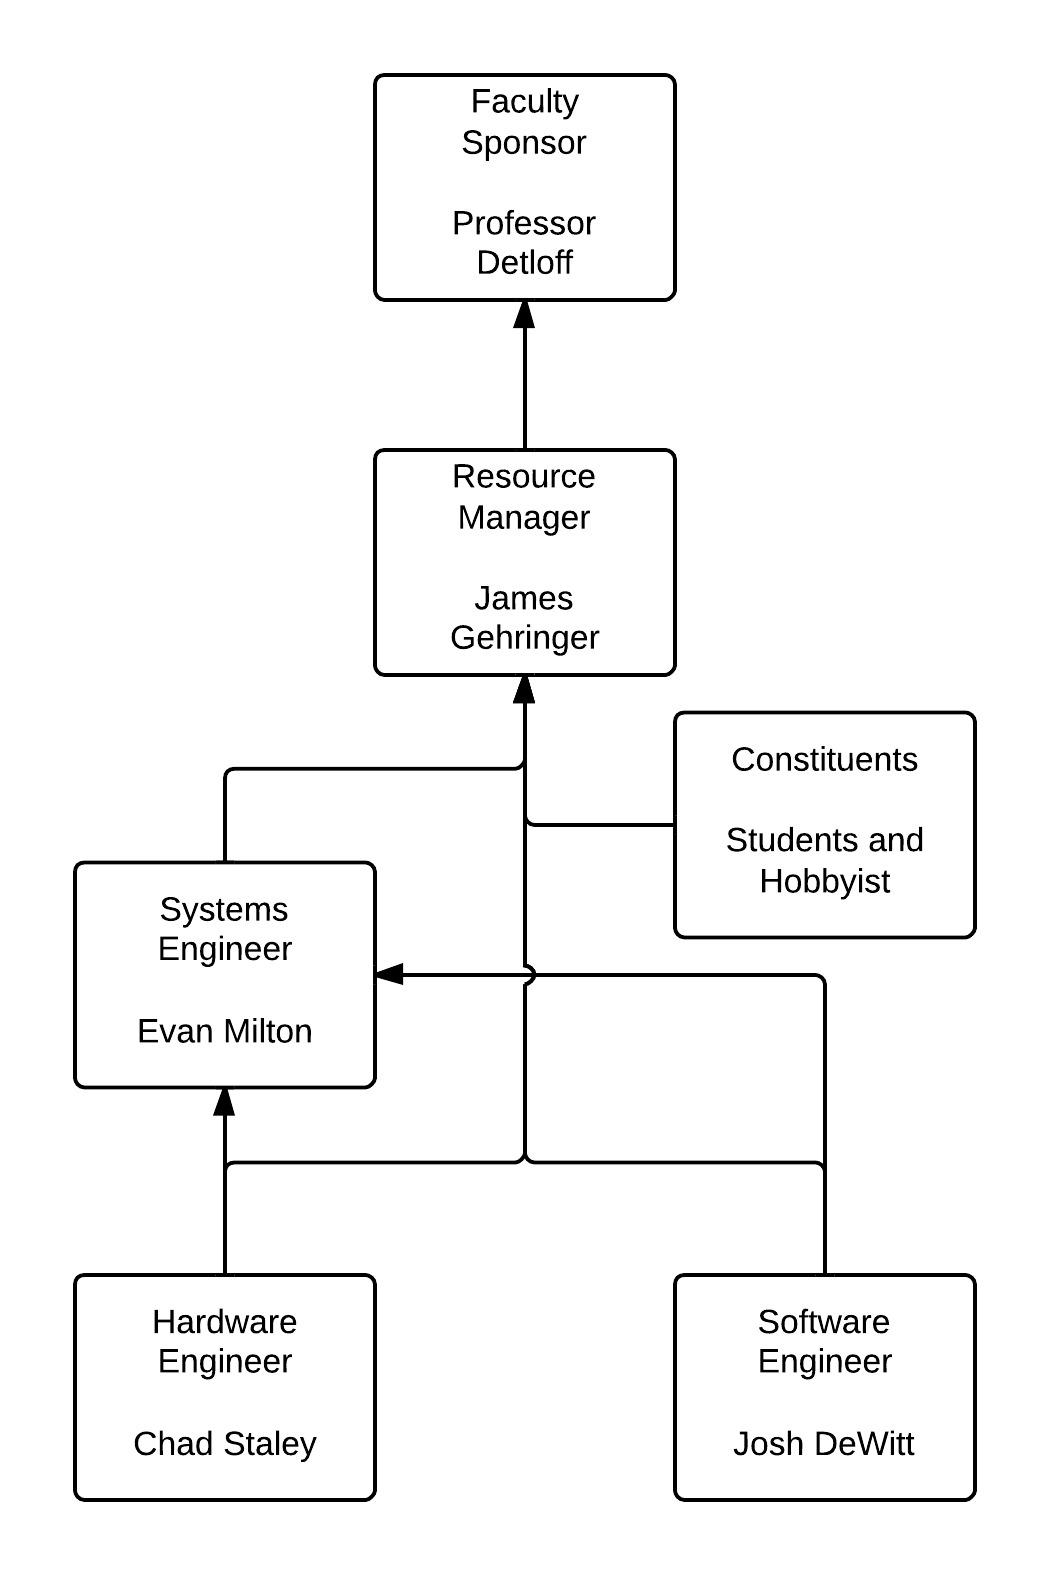
\includegraphics[width=0.6\textwidth]{shc.jpeg}
\caption{Stakeholder Chart}
\label{fig:Stakeholder Chart}
\end{figure}
The Stake Holder chart has been reviewed and updated to the Figure 7.1.
These are all the parties that are currently invested in the project. 
If more parties become invested, then the organization and chart will be revisited. 

Communication techniques being used are successful in keeping all involved informed.
As the project progresses, more face-to-face team meetings will occur.
In the event that communication channels start to break down, a team meeting will be called and new processes will be evaluated. 

Resources needed have been reduced. 
The \gls{cnc} Interface does not need mechanical parts, eliminating many of the hardware resources.

\pagebreak
\section{Linear Responsibility Chart}
\begin{longtable}{|c|m{1.8cm}|m{1.8cm}|>{\centering}m{1.8cm}|m{1.8cm}|m{1.8cm}|m{2.5cm}|}
	\caption{Linear Responsibility Chart}
	\label{table:primary} \\
	\hline \textbf{\gls{wbs} ID} & \textbf{Josh \newline DeWitt} & \textbf{James \newline Gehringer} & \textbf{Evan Milton} & \textbf{Chad \newline Staley} & \textbf{Herb Detloff} \\ \hline
	\endfirsthead
	\multicolumn{7}{c}{\tablename\ \thetable\ -- \textit{Continued from previous page}} \\ \hline
	 \textbf{\gls{wbs} ID} & \textbf{Josh \newline DeWitt} & \textbf{James \newline Gehringer} & \textbf{Evan Milton} & \textbf{Chad \newline Staley}& \textbf{Herb Detloff}
	\endhead 
	\multicolumn{7}{r}{\textit{Continued on next page}} \\
	\endfoot \hline
	\endlastfoot


	\hline 1 & \multicolumn{6}{c|}{Electrical Components} \\ \hline
	1.1  &4&4&2&1&  \\ \hline
	1.2  &4&4&1&2&  \\ \hline
	1.2.1&4&4&1&2&  \\ \hline
	1.2.2 &4&4&1&2&  \\ \hline
	1.2.3 &4&4&1&2&  \\ \hline
	1.2.4 &4&4&1&2&  \\ \hline
	1.3  &4&4&2&1&\\ \hline
	1.4  &4&4&1&2&   \\ \hline
	\hline 2 & \multicolumn{6}{c|}{Control Software} \\ \hline
	2.1  &1&2&4&4&   \\ \hline
	2.1.1 &1&2&4&4 &  \\ \hline
	2.1.2 &1&2&4&4&  \\ \hline
	2.2  &1&2&4&4& \\ \hline
	2.2.1 &1&2&4&4&   \\ \hline
	2.2.2 &1&2&4&4&   \\ \hline
	2.3 &1&2&4&4& \\ \hline
	2.3.1 &1&2&4&4&  \\ \hline
	2.3.2 &1&2&4&4&  \\ \hline
	2.4  &1&2&4&4&\\ \hline
	2.4.1 &1&2&4&4& \\ \hline
	2.4.2 &1&2&4&4& \\ \hline
	2.5 &2&3&1&4& \\ \hline
	\hline 3 & \multicolumn{6}{c|}{Interface Software} \\ \hline
	3.1  &1& 2&4 &4 & \\ \hline
	3.2  &1& 2& 4& 4& \\ \hline
	3.3 & 1&2& 4& 4& \\ \hline
	3.4  &2&1 & 4&4 &\\ \hline
	\hline 4 & \multicolumn{6}{c|}{System Testing} \\ \hline
	4.1  &3&3&2&1&6\\ \hline
	4.2  &1&2&4&4&6\\ \hline
	4.3  &3&3&2&1&6\\ \hline
	4.4  &4&3&1&2&6\\ \hline
	4.5  &3&4&1&2&6\\ \hline
	\hline 5 & \multicolumn{6}{c|}{Integration Testing} \\ \hline
	5.1  &2&1&4&4&6\\ \hline
	5.2  &1&4&2&3&6\\ \hline
	5.3  &3&4&1&2&6\\ \hline
	5.4  &3&4&2&1&6\\ \hline
	\hline 6 & \multicolumn{6}{c|}{Unit Testing} \\ \hline
	6.1  &1&2&3&4& \\ \hline
	6.2  &4&3&2&1& \\ \hline
	6.3  &4&3&1&2& \\ \hline
	\hline 7 & \multicolumn{6}{c|}{Product Management} \\ \hline
	7.1 &2&1&2&2&  \\ \hline
	7.2  &4&1&2&3&  \\ \hline
	7.3  &2&1&4&3&  \\ \hline
	7.4  &2&1&2&2&  \\ \hline
	7.5 &4&1&2&3&  \\ \hline
	7.6 &2&1&2&2&\\ \hline
	7.7 &2&1&2&2&4\\ \hline
\end{longtable}
Key:
\begin{tabular}{l l l}
	1 - Primary Responsibility & 2 - Support Work & 3 - Must be Consulted \\
	4 - May be Consulted & 5 - Review & 6 - Final Approval \\
\end{tabular}
\section{Activity on Node Dependency Network}
\begin{figure}[H]
\centering
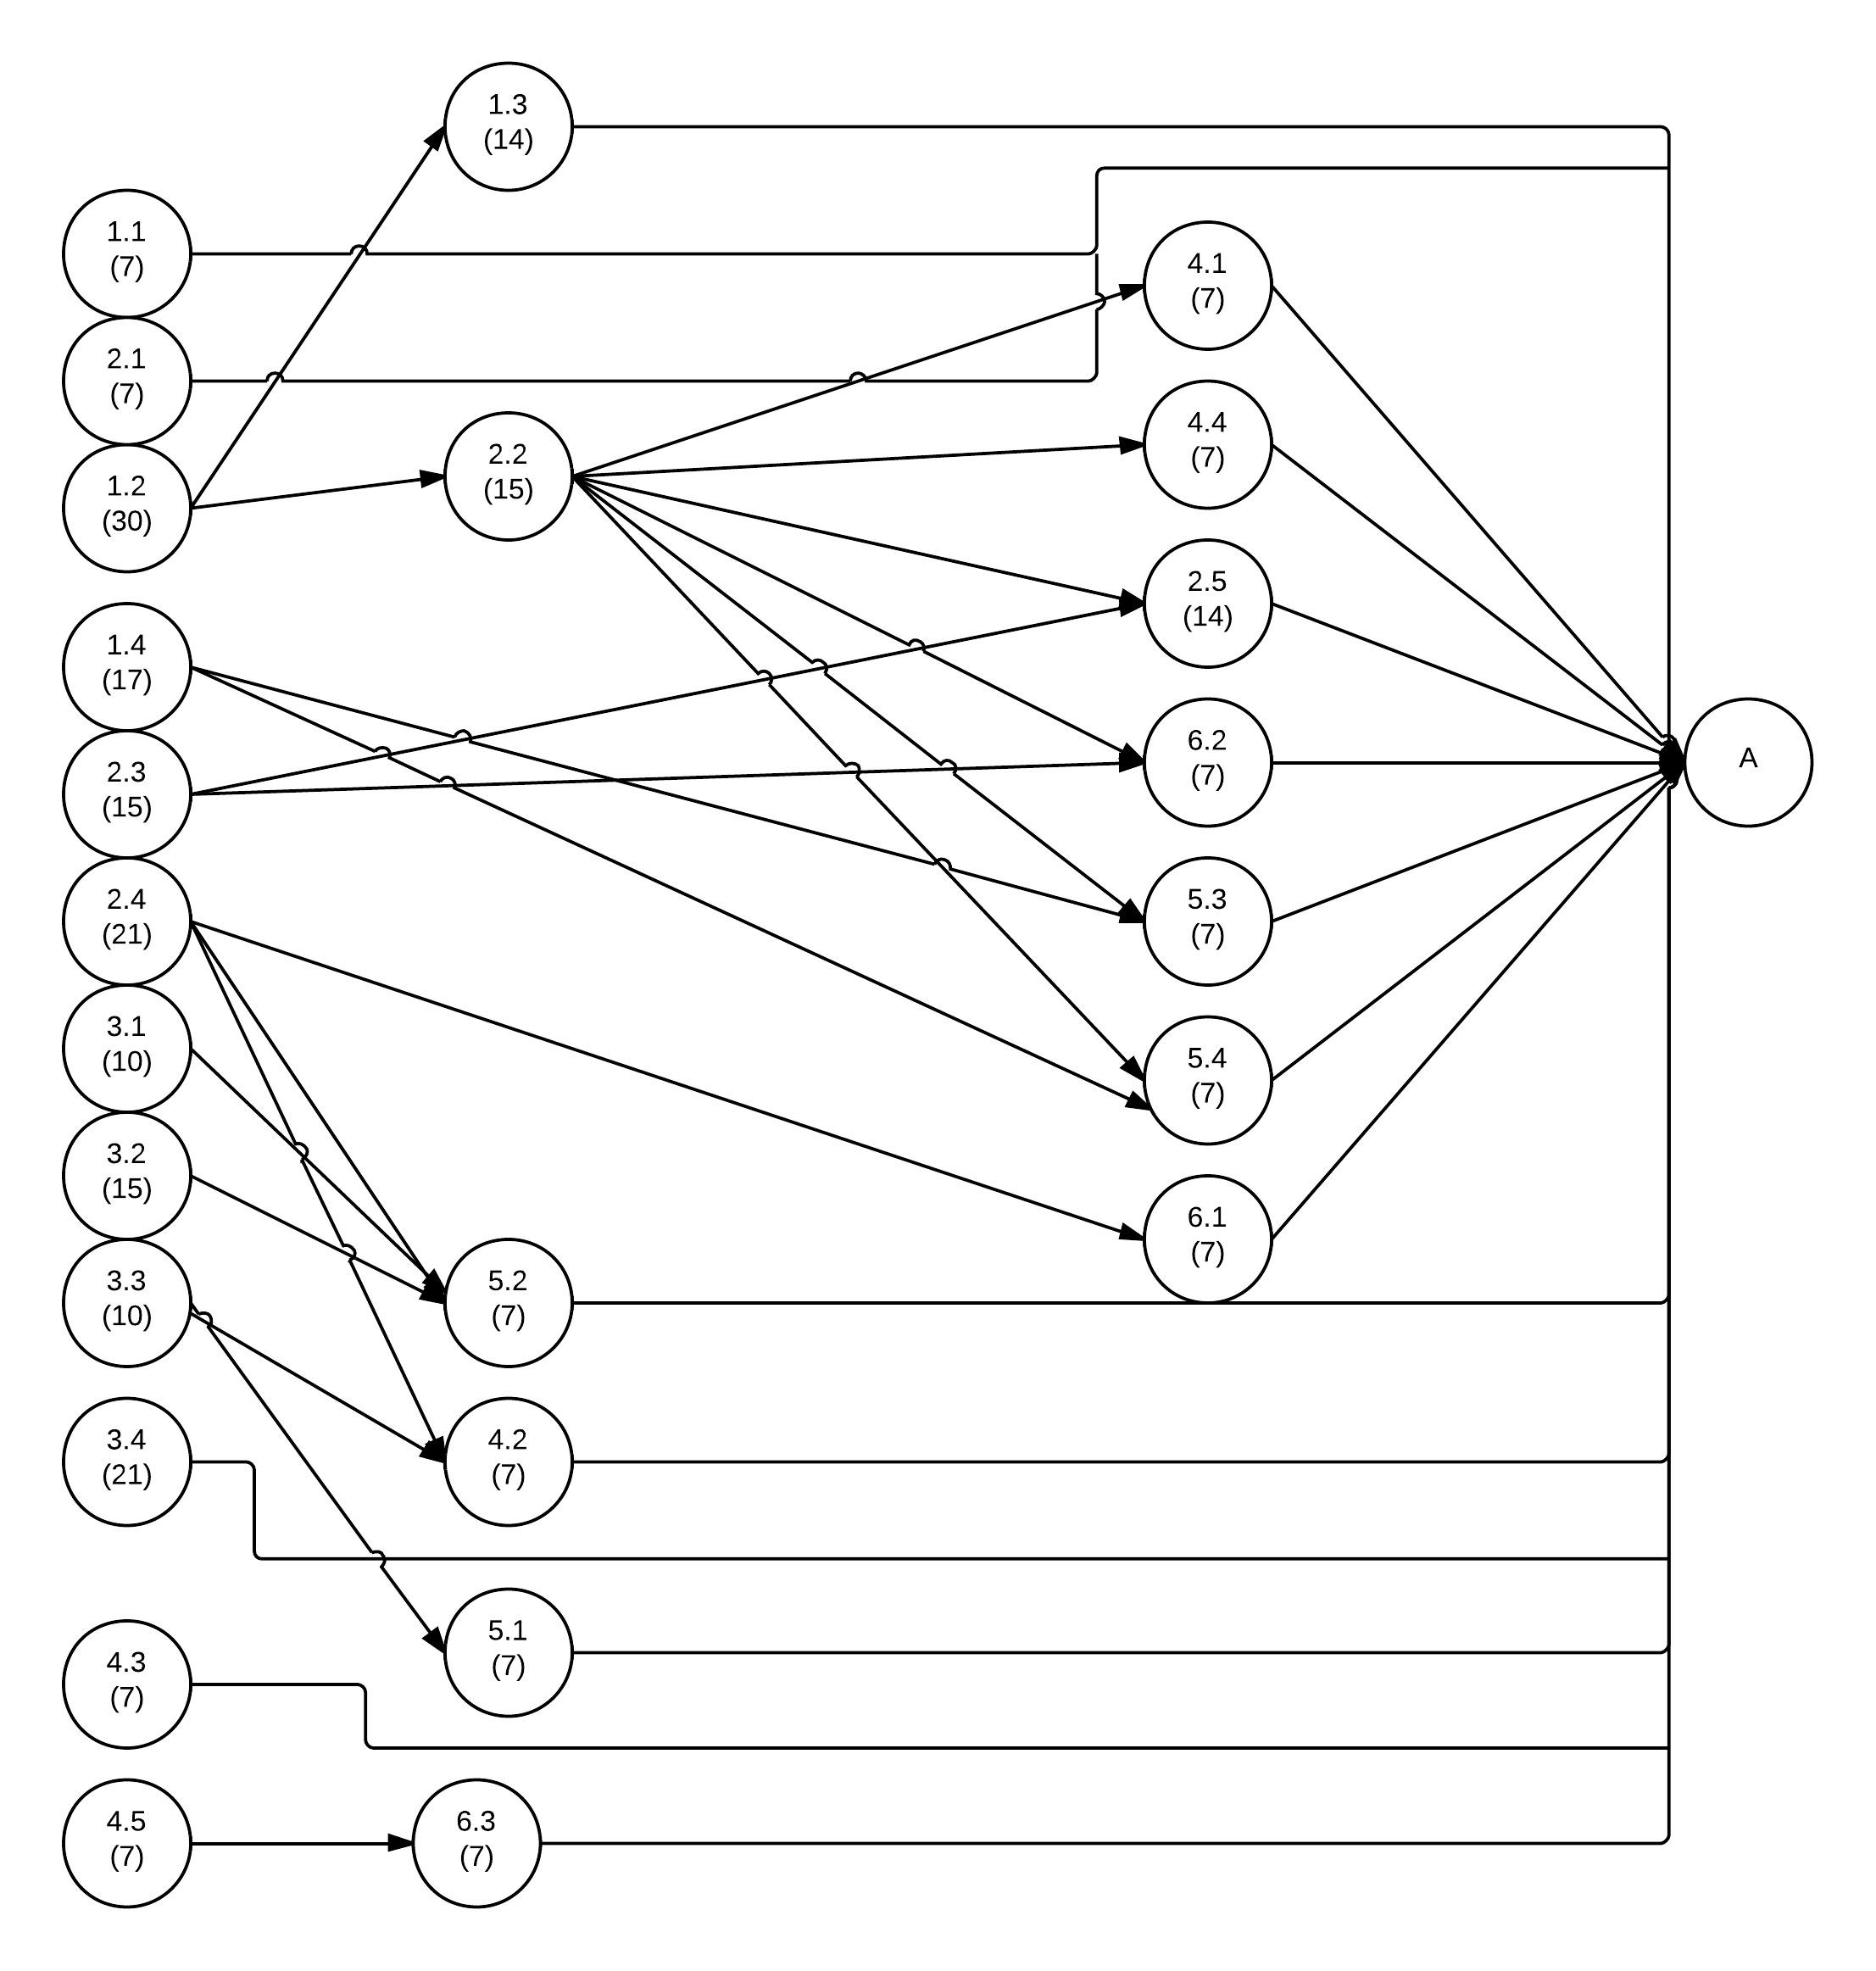
\includegraphics[width=1\textwidth]{AON.jpeg}
\caption{Activity on Node}
\label{fig:Activity on Node}
\end{figure}
\section{Gantt Chart Schedule}
\begin{figure}[H]
\centering
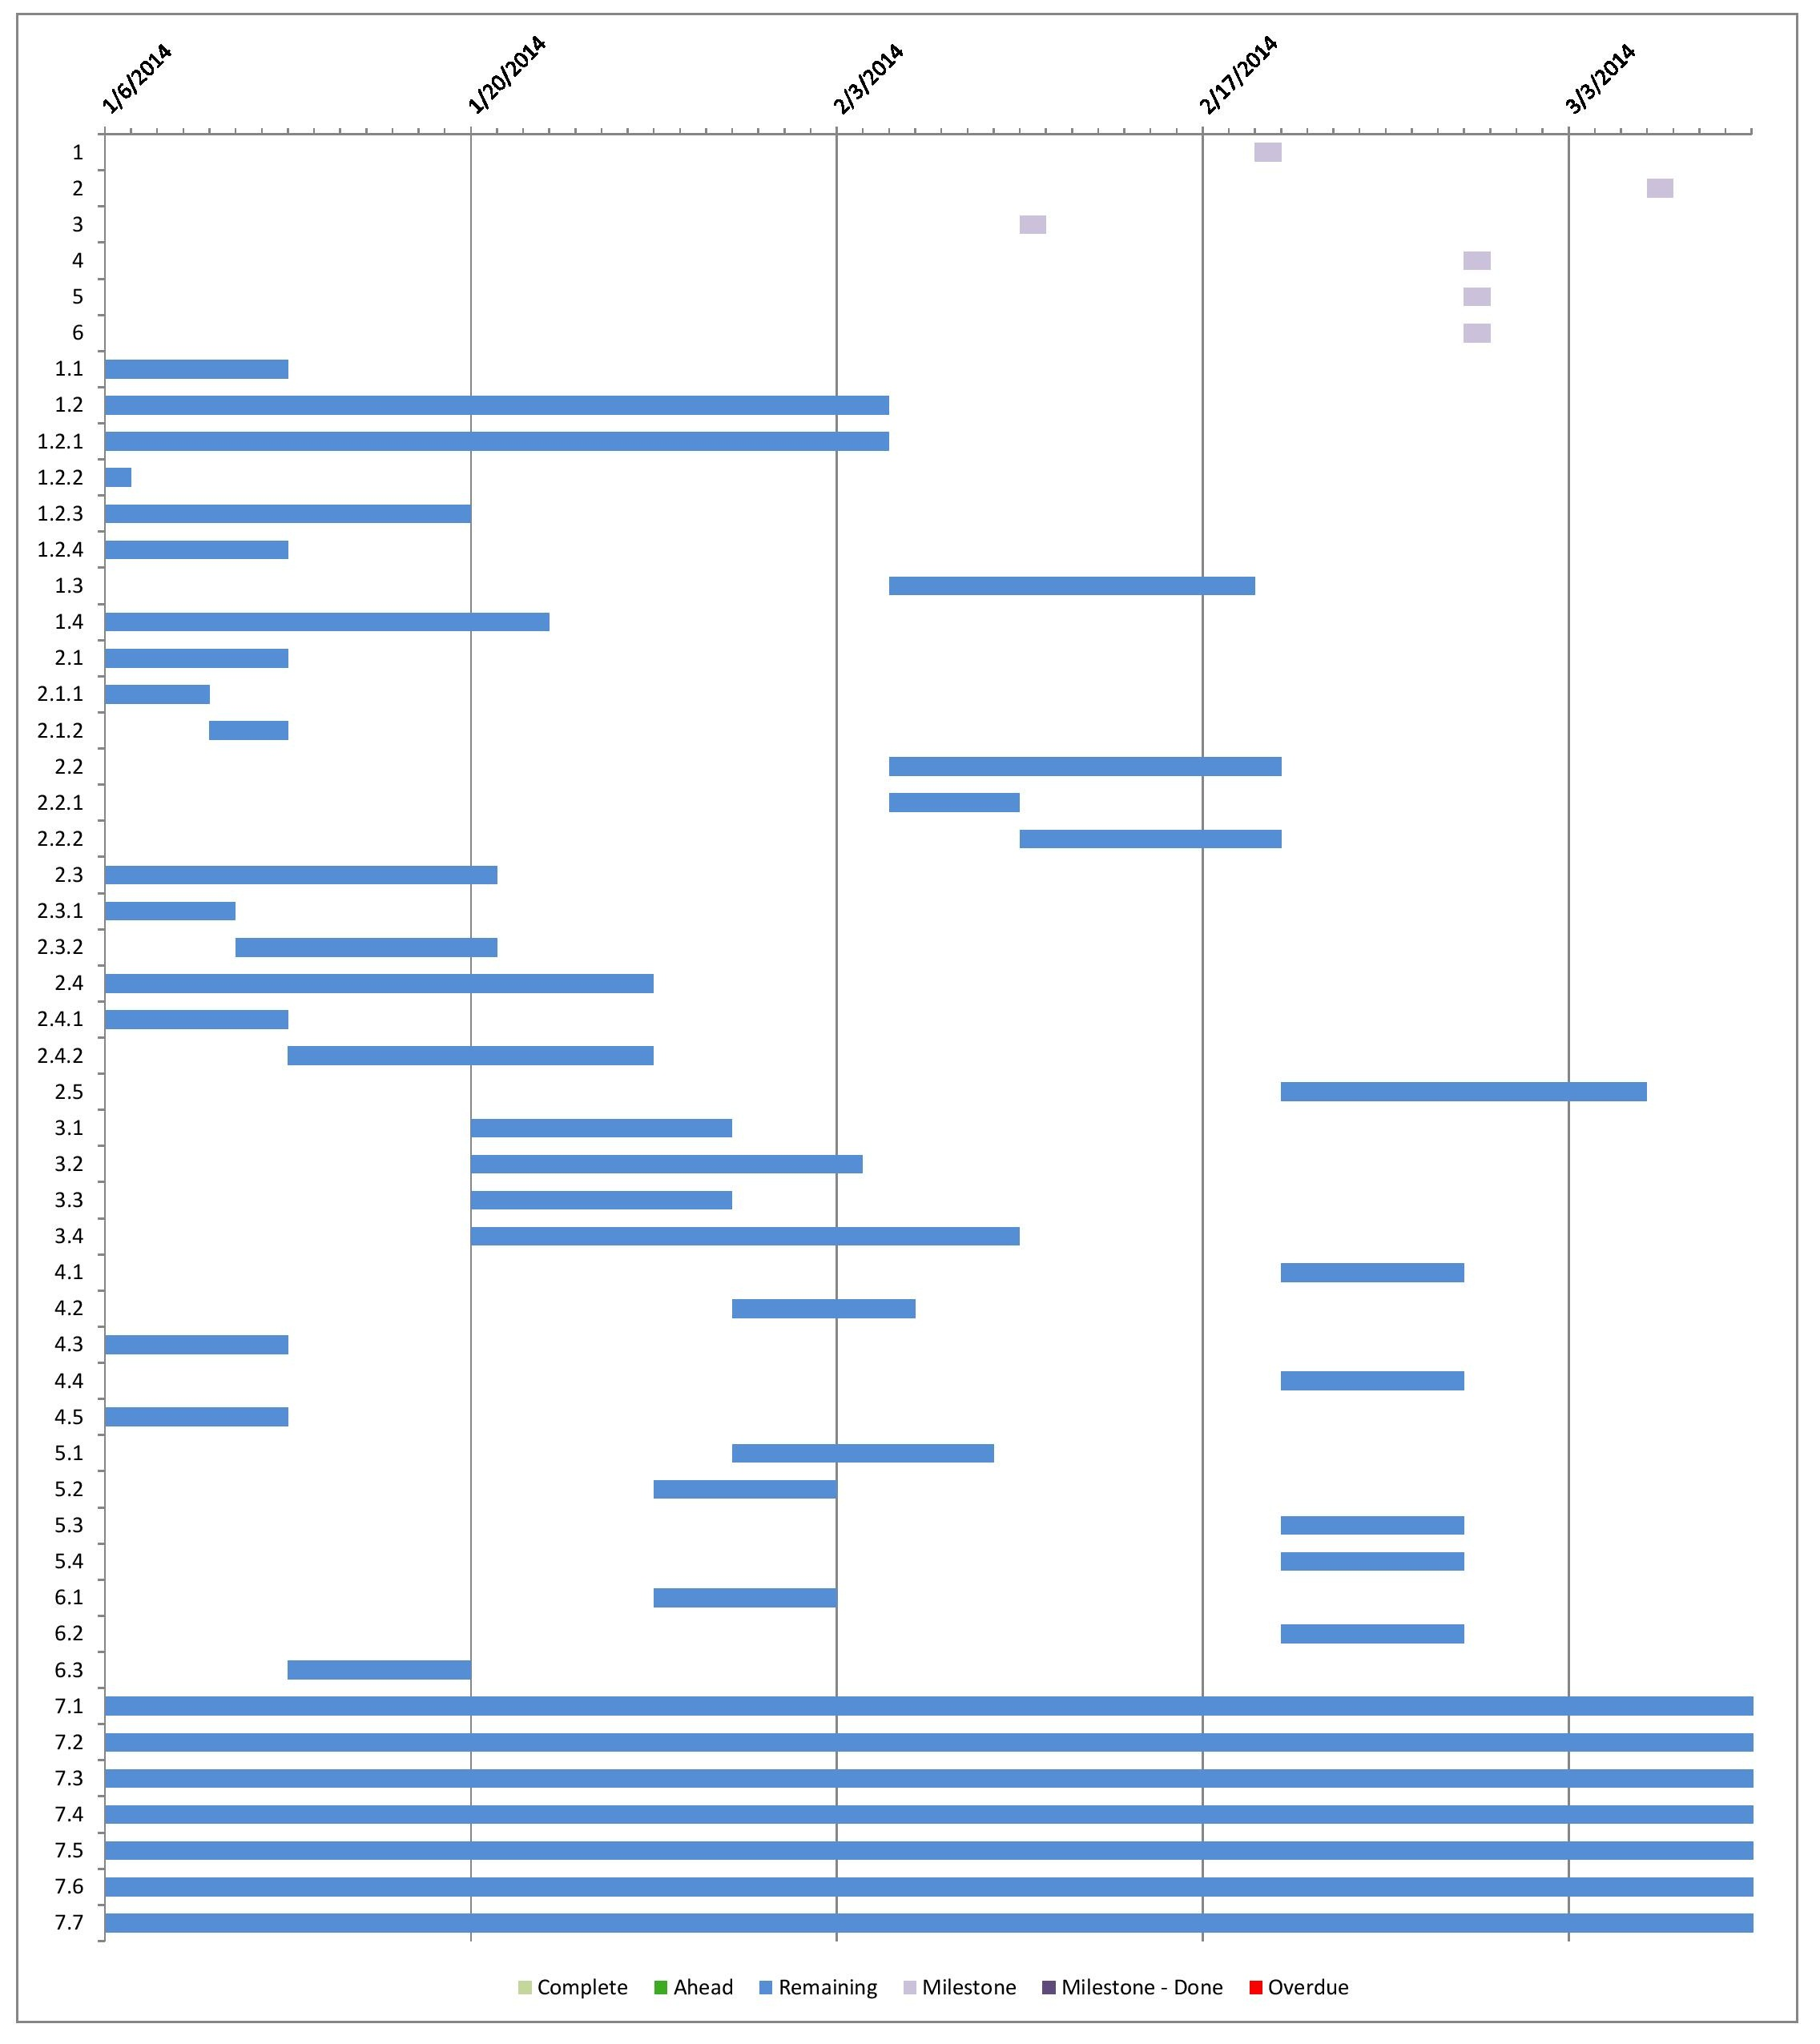
\includegraphics[width=1\textwidth]{gantt.jpg}
\caption{Activity on Node}
\label{fig:Activity on Node}
\end{figure}
\subsection{Landmark Schedule}
Each landmark is marked on the Gantt Chart with a triangle.
\subsection{Critical Design Review Schedule}
Critical design reviews will happen every two weeks, marked on the Gantt Chart by the solid vertical red lines.
Critical design review will end after 6 weeks. By this point the critical parts of the project should be finalized. 
\subsection{\gls{wbs} and \gls{lrc} Review and Update Schedule}
Chart updates will happen every two weeks, denoted by both the solid and dashed vertical red lines.
\section{Budget}
\begin{longtable}{|>{\centering}m{3.0cm}|>{\centering}m{1.8cm}|>{\centering}m{1.8cm}|>{\centering}m{1.8cm}|>{\centering}m{1.8cm}|>{\centering}m{2.3cm}|m{1.8cm}|}
	\caption{Budget}
	\label{table:primary} \\
	\hline \textbf{Item} & \textbf{Required} & \textbf{Purchase} & \textbf{Cost} & \textbf{Total} & \textbf{Specification} &\textbf{Supplier}\\ \hline
	\endfirsthead
	\multicolumn{7}{c}{\tablename\ \thetable\ -- \textit{Continued from previous page}} \\ \hline
	 \textbf{Item} & \textbf{Required} & \textbf{Purchase} & \textbf{Cost} & \textbf{Total} & \textbf{Specification} &\textbf{Supplier}
	\endhead 
	\multicolumn{7}{r}{\textit{Continued on next page}} \\
	\endfoot \hline
	\endlastfoot

	Motor Driver Unit&4 &5& \$14.95& \$74.75&DRV 8825&Pololu\\ \hline
	Motor Controller Development Board&1&2&\$35.00&\$70.00& RasPi 512MB&Newark\\ \hline
	Master Controller Development Board&1&2&\$35.00&\$70.00&MSP430 FR5739 Dev Kit&TI\\ \hline
	Peripheral Components&1&2&\$30.00&\$60.00&Misc on-board electronics&Tayda\\ \hline
	Motor Connection Hardware&4&5&\$10.00&\$50.00&8 Pin Mil-Spec Connectors&eBay\\ \hline
	Power Supply Unit&1&2&\$25.00&\$50.00&10A, Switching PSU&eBay\\ \hline
	Testing Materials&1&1&\$50.00&\$50.00&Stuff to carve up&Lowes\\ \hline
	Enclosure&1&1&\$50.00&\$50.00&Fabricate in house&Lowes\\ \hline
	Monitor for\\Master Controller&1&1&\$35.00&\$35.00&HDMI compatible (used)&GoodBytes\\ \hline
	Cabling \& Test Harness&1&2&\$10.00&\$20.00&Wire is expensive&eBay\\ \hline
	Voltage Regulation&2&3&\$6.00&\$18.00&DC-DC Converter&eBay\\ \hline
	Total &&&&\$547.75&&\\ \hline
\end{longtable}
\section{Engineering Hours}

\begin{table}[H] 
\caption{Engineering Hours}
	\label{table:engineeringhours}
	\centering 
\begin{tabular}{|r|c|}
	
	\hline Josh DeWitt&150\\ \hline
	James Gehringer&150\\ \hline
	Evan Milton&150\\ \hline
	Chad Staley&150\\ \hline
	Total&600\\ \hline
\end{tabular}
\end{table} 

\end{document}
